\documentclass[sigconf]{acmart}
\usepackage[utf8]{inputenc}
\usepackage[english]{babel}
\usepackage{lmodern}
\usepackage[T1]{fontenc}    

\usepackage{color}
\usepackage{subcaption}

\usepackage{amssymb}
\usepackage{amsmath}
\DeclareMathOperator*{\argmin}{arg\,min\,}
\DeclareMathOperator*{\argmax}{arg\,max\,}
\DeclareMathOperator{\sign}{sign}
\DeclareMathOperator{\loss}{loss}
\DeclareMathOperator{\softmax}{softmax}\DeclareMathOperator{\softplus}{softplus}

\DeclareMathOperator{\EX}{\mathbb{E}}% expected value

\newcommand{\myvec}[1]{\boldsymbol{#1}}
\newcommand{\minimize}{\text{minimize}}
\newcommand{\optimize}[4]{\begin{aligned}
& \underset{#2}{#1}
& & #3 \\
& \text{subject to}
& & #4
\end{aligned}}
\usepackage{natbib}
\setcitestyle{square, comma, numbers,sort&compress, super}

\usepackage{tikz}
\usetikzlibrary{positioning}
\usepackage{tikz-qtree}
\usetikzlibrary{arrows, calc, decorations.pathreplacing, angles, quotes, positioning}
\usetikzlibrary{shapes.geometric}
\usetikzlibrary{chains}

% configure acm template to a minimalistic version
\setcopyright{none}
\settopmatter{printccs=false, printacmref=false, printfolios=false}
\renewcommand\footnotetextcopyrightpermission[1]{} % removes footnote with conference information in first column
\pagestyle{plain} % removes running headers

\widowpenalty
\clubpenalty

\begin{document}
% Title portion
\title{InformatiCup 2019}

\author{Jonas Möller}
\affiliation{%
	\institution{TU Braunschweig}
}
\email{jo.moeller@tu-braunschweig.de}

\author{Lukas Pirch}
\affiliation{%
	\institution{TU Braunschweig}
}
\email{l.pirch@tu-braunschweig.de}

\maketitle

\section{Introduction}

In recent years, Machine Learning algorithms have received much attention due to their efficiency in solving otherwise difficult classification tasks.
Amongst others, there are applications in spam filtering \cite{ruan2010three, clark2003neural}, malware detection \cite{dahl2013large}, natural language processing \cite{collobert2008unified} and image classification \cite{simonyan2014very, he2016deep}.
In the latter domain, deep neural networks (DNNs) and especially convolutional neural networks (CNNs) have become very popular.
However, recent research has also shown that these ML algorithms are vulnerable to crafting malicious inputs, called \enquote{adversarial examples}.
These inputs are created by an attacker with the intention of tricking the machine learning system into misclassifying.
\citet{szegedy2013intriguing} were the first to explore this kind of evasion attack aimed at finding unnoticeable modifications to a valid input sample such that it is misclassified by the DNN but still looks the same to a human observer.

This year's InformatiCup challenge revolves around a related topic: The task is to generate images which do not look like traffic signs but are classified as such by a remote model with a high confidence (90\%).
Because image classification is used for self-driving cars which automatically detect and classify traffic signs, this issue is equally topical and relevant.
It is an essential goal to prevent self-driving cars from being mislead by these adversarial examples since this could potentially endanger human lives.
Considering a situation in which someone places a sticker on the back of a lorry which looks benign to humans but is classified as a yield sign by a car, the criticality of this topic becomes very clear.
This motivates exploring different kinds of attacks against ML algorithms in order to better understand the vulnerabilities, paving the way for setting up effective defenses.
Adversarial Examples themselves are an active research direction and though there exist a plethora of attacks, it's neither clearly established why adversarial examples exist nor how to effectively defend against them.

One of the most prominent projects for benchmarking defenses is the CleverHans project in which several state-of-the-art attacks are included \cite{papernot2016cleverhans}.
By leveraging these existing algorithms and creating custom extensions to them, this work contributes to a better understanding of how adversarial examples can be generated and physically applied.
For example, perturbations are only valid for a single image in most cases, which has been taken from a certain angle.
In the situation of a self-driving car passing by an adversarial example, this would only trigger in a fraction of a second.
To cover a more realistic scenario, we implemented a modified attack which makes these adversarial examples robust against being seen from different angles.

On a more detailed level, the scenario of this challenge is similar to the \enquote{rubbish class examples} described by \citet{szegedy2015explaining}, which are images that a human would not assign any of the given classes.

An obstacle in the competition is the access to the remote model, which is only accessible via a web interface,
reporting the top five most-likely classes and their confidences for a given image.
This means that the architecture, the weights and the training hyperparameters are unknown, which are critical to most attacks that generate adversarial examples.
This impediment is overcome by \citet{papernot2017practical} who turn the limited access into a white box model.
Therefore, the challenge of this task lies in combining multiple insights of adversarial research and applying them in a real-world situation.

\begin{figure}
\vspace{4ex}
\centering
\begin{subfigure}{.19\linewidth}
  \centering
  
\includegraphics[width=0.7\linewidth]{imgs/octocat}
\end{subfigure}
\begin{subfigure}{.19\linewidth}
  \centering
  
\includegraphics[width=0.7\linewidth]{imgs/4}
\end{subfigure}
\begin{subfigure}{.19\linewidth}
  \centering
  
\includegraphics[width=0.7\linewidth]{imgs/4_real}
\end{subfigure}

\begin{subfigure}{.19\linewidth}
  \centering
  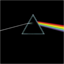
\includegraphics[width=0.7\linewidth]{imgs/darkside}
\end{subfigure}
\begin{subfigure}{.19\linewidth}
  \centering
  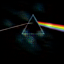
\includegraphics[width=0.7\linewidth]{imgs/7}
\end{subfigure}
\begin{subfigure}{.19\linewidth}
  \centering
  
\includegraphics[width=0.7\linewidth]{imgs/7_real}
\end{subfigure}

\begin{subfigure}{.19\linewidth}
  \centering
  
\includegraphics[width=0.7\linewidth]{imgs/gi}
\end{subfigure}
\begin{subfigure}{.19\linewidth}
  \centering
  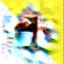
\includegraphics[width=0.7\linewidth]{imgs/10}
\end{subfigure}
\begin{subfigure}{.19\linewidth}
  \centering
  
\includegraphics[width=0.7\linewidth]{imgs/10_real}
\end{subfigure}
\caption{Excerpt from our results: Each row contains from left to right an input image, an adversarial example and a typical target class image.}
\label{fig:eyecatcher}
\end{figure}

An excerpt from our results is shown in Figure \ref{fig:eyecatcher}. 
Each row contains the source image on the left, the result from the attack in the center and an image of the falsely classified label by the remote model on the right.
A thorough explanation of how these example have been created as well as a discussion about the result quality can be read in the remainder of this paper, which is organized as follows:

At the beginning, we provide the background information required to understand our approach in Section~\ref{sec:background} and describe the prevalent threat model in Section~\ref{sec:threatmodel}.
After that, the theoretical approach as well as the software development and testing strategy are explained in Section~\ref{sec:methodology}.
Our implementation's architecture is presented in Section~\ref{sec:arch}.
Section~\ref{sec:results} shows our submitted images with a brief explanation of our results which are thereafter evaluated in Section~\ref{sec:evaluation}.
At the end, we present possible future extensions in Section~\ref{sec:extensibility}, discuss the general quality of our solution in Section~\ref{sec:discussion} and conclude our results in Section~\ref{sec:conclusion}.
%!TEX root = paper.tex"`

\section{Background}\label{sec:background}

\begin{figure}
\centering
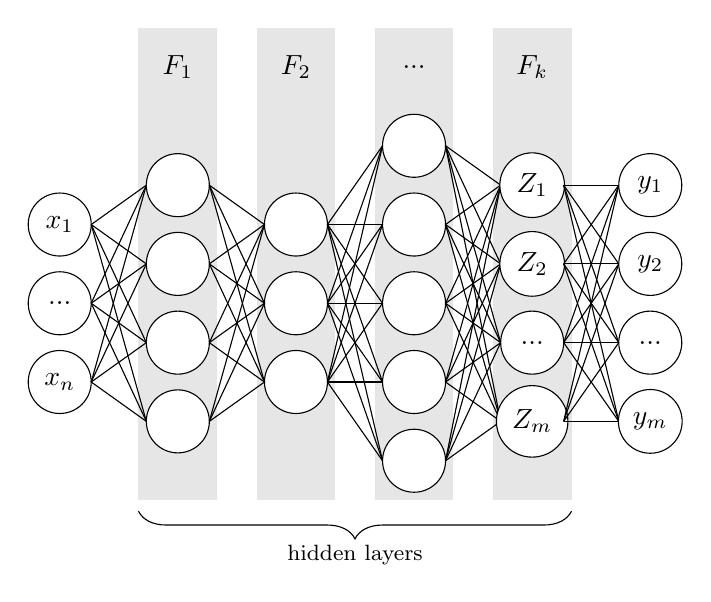
\begin{tikzpicture}[yscale=-1]
\tikzset{neuron/.style={
    shape=circle,
    fill=white,
    draw,
    minimum size=0.8cm
}}

%\draw[step=1cm,gray,very thin,fill=white] (0,0) grid (8,6);

\fill[opacity=0.2,fill=gray] (1,-0.5) rectangle (2,5.5);

\fill[opacity=0.2,fill=gray] (2.5,-0.5) rectangle (3.5,5.5);

\fill[opacity=0.2,fill=gray] (4,-0.5) rectangle (5,5.5);

\fill[opacity=0.2,fill=gray] (5.5,-0.5) rectangle (6.5,5.5);

\node[neuron] at (0, 2) {$x_1$};
\node[neuron] at (0, 3) {...};
\node[neuron] at (0, 4) {$x_n$};

\foreach \x in {1,...,3}{
	\draw (0.4, \x+1) -- (1.1,1.5);	\draw (0.4, \x+1) -- (1.1,2.5);
	\draw (0.4, \x+1) -- (1.1,3.5);
	\draw (0.4, \x+1) -- (1.1,4.5);
}

\node[] at (1.5, 0) {$F_1$};
\foreach \x in {2,...,5}{
	\node[neuron] at (1.5, \x-0.5) {};
	\draw (1.9, \x-0.5) -- (2.6,2);
	\draw (1.9, \x-0.5) -- (2.6,3);
	\draw (1.9, \x-0.5) -- (2.6,4);
}

\node[] at (3, 0) {$F_2$};
\foreach \x in {2,...,4}{
	\node[neuron] at (3, \x) {};
	\draw (3.4, \x) -- (4.1,1);	\draw (3.4, \x) -- (4.1,2);
	\draw (3.4, \x) -- (4.1,3);
	\draw (3.4, \x) -- (4.1,4);
	\draw (3.4, \x) -- (4.1,5);
}

\node[] at (4.5, 0) {...};
\foreach \x in {1,...,5}{
	\node[neuron] at (4.5, \x) {};
	\draw (4.9, \x) -- (5.6,1.5);	\draw (4.9, \x) -- (5.6,2.5);
	\draw (4.9, \x) -- (5.6,3.5);
	\draw (4.9, \x) -- (5.6,4.5);
}

\draw [decorate,decoration={brace,amplitude=10pt,mirror,raise=4pt},yshift=0pt]
(1,5.5) -- (6.5,5.5) node [black,midway,yshift=-0.7cm] {\footnotesize hidden layers};

\node[] at (6, 0) {$F_k$};
\foreach \x in {1,...,2}:
	\node[neuron] at (6, \x+0.5) {$Z_\x$};
\node[neuron] at (6, 3.5) {...};
\node[neuron] at (6, 4.5) {$Z_m$};

\foreach \x in {1,...,4}{
	\draw (6.4, \x + 0.5) -- (7.1,1.5);
	\draw (6.4, \x + 0.5) -- (7.1,2.5);
	\draw (6.4, \x + 0.5) -- (7.1,3.5);
	\draw (6.4, \x + 0.5) -- (7.1,4.5);
}

\foreach \x in {1,...,2}:
	\node[neuron] at (7.5, \x+0.5) {$y_\x$};
\node[neuron] at (7.5, 3.5) {...};
\node[neuron] at (7.5, 4.5) {$y_m$};
\end{tikzpicture}
\caption{Visualization of a neural network}
\label{fig:neuralnetwork}
\end{figure}

This section provides the general background knowledge required to understand the remainder of this paper.
In addition, the basic notation which is going to be used later is defined.
A reader familiar with the domain of adversarial machine learning is suggested to continue reading at Subsection~\ref{sec:threatmodel}.

\subsection{Deep Neural Networks}\label{subsec:dnn}
Deep neural networks (DNNs) are a form of machine learning algorithms based on a concept loosely analogous to the human brain.
On a conceptual level, DNNs take a vector of numbers as an input and assign it a output vector which represents the probability for each class which has been considered during training.
Thus, real-world input objects need to be transformed to a so called \enquote{feature space}, their mathematical abstraction that can be passed to the DNN.
In the context of image recognition, this relates to taking each input pixel's color channel as an input feature.
Having a look on the inner structure, neural networks consist of a set of nodes (\enquote{neurons}), which are organized in successive layers.
Each neuron is represented by a mathematical function taking a weighted sum of inputs and returning the value of a previously specified activation function.
Currently, the sigmoid function $H : x \mapsto \frac{1}{1 + e^{-x}}$ and the rectified linear unit (ReLU) function $H : x \mapsto max(0, x)$ are the most common activation functions in practice.
In a fully connected architecture, the activation of each neuron is affected by each output of the previous layer.
More precisely, each neuron's output is defined as the weighted sum of all previous layer's outputs, subsequently transformed by an activation function.
The output of the final layer is transformed using a softmax function $\sigma : x \mapsto \frac{e^{x_i}}{\sum_{j=1}^{N} e^{x_j}}$ for $\forall i \in N$ with $N$ as the number of dimensions.
Simply put, this function returns a confidence score by mapping each value to the range $(0, 1]$ and scaling the output such that the sum of all outputs is equal to one.
This is the previously mentioned output probability assigned to a certain input.
The quality of a DNN's classification is determined by a loss function, which indicates the distance of a given output from the optimal solution.

Before a network can be used, it needs to be trained.
The training phase includes repeatedly feeding given input-output pairs through the network, evaluating the output using the loss function and adjusting the weights.
For the latter, a backpropagation algorithm is used which decreases the weights of previous layers that contributed most to the loss, effectively increasing the relative impact of those weights contributing to a correct classification.
At the beginning, the weights are usually random and after multiple training iterations (epochs), the network starts to infer a functional dependency from the training samples.
The set of learned weights is referred to as a model $\theta$.
Furthermore, there are parameters that are not directly related to the learned model but affect the learning process.
These are referred to as \enquote{hyperparameters}.
Two examples for such a hyperparameter are the learning rate and the selected optimizer.

Additionally, Convolutional Neural Networks (CNNs) are going to be examined in the course of this project.
They are an extension of regular DNNs and have proven to work well in the domain of image classification \cite{matsugu2003subject, krizhevsky2012imagenet}.
The key difference here is that there are additional types of layers.
Convolution layers perform a special operation taking a spatial sliding window (called \enquote{receptive field} or \enquote{filter}) and returning its activation.
Depending on the architecture, multiple filters may be used.
After the convolution layer, a pooling layer reduces the dimensionality using a specified downsampling function.
For example, the \enquote{Max Pooling} returns the maximum value in a spatial neighborhood.
As a result, the CNN is able to recognize edges and other spatial characteristics of an image without any preprocessing.

\subsection{Distance Metrics}\label{subsec:metrics}
The definition of distances in a feature space is crucial for a successful classification.
In the domain of image recognition, it quantifies how different two images are.
Selecting an appropriate distance metric is relevant when perturbing an image because each attack algorithm is optimized under a certain metric.
Evaluating the suitability of a given metric in this context however is not trivial, because it depends more on how humans perceive images than on how big their differences are in theory.
An attack might yield good results according to a specific metric while a human observer would disagree on this.
To give a basic notion of distance metrics, the three most commonly used metrics are briefly presented below.

The $L_0$ distance between two images counts how many pixels are different from each other.
Using this metric is based on the simple idea that images look more different the more pixels have been altered.
An example of an attack that uses this metric is the Jacobian-based Saliency Map Attack \cite{papernot2016limitations}.
In contrast to that, the $L_\infty$ norm measures the maximum difference of any pixel.
This metric reflects the situation in which single strongly modified pixels are immediately recognizable.
For instance, the Fast-Gradient Sign Method is optimized under this distance metric~\cite{szegedy2015explaining}.
Finally, there is the $L_2$ norm which appears to be the most beneficial when creating adversarial examples.
It computes the square root of the pixel-wise squared sum of differences of two images.
This is equivalent to a distance in euclidean space which gives a natural sense of the dissimilarity between two images.

\subsection{Notation}\label{subsec:notation}
In the remainder of this document, different aspects related to Machine Learning are going to be analyzed and discussed.
The utilized notation is briefly presented in this subsection.

%TODO define only notation that is actually used
% perturbed image's distance delta
% norm, L2-norm
%!TEX root = paper.tex

\section{Methodology}\label{sec:methodology}

In this section, we present our theoretical approach to attacking the remote model and our practical methodology for developing a suitable software.
The general idea is to train a local model which approximates the behavior of the remote model.
Thus, we describe first how we turn the remote black-box oracle into a local white-box model in subsection~\ref{subsec:modelstealing}.
Afterwards, we attack the local model and expect the generated image to also fool the remote model, depending on our approximation quality.
Therefore, we introduce the attacks for generating adversarial examples in the subsequent parts of this section.
Finally, we present our software developing methodology in subsection~\ref{subsec:sw_development}.

\subsection{Model Stealing}\label{subsec:modelstealing}

The attacks which are introduced later in this section assume white-box access to a target model (i.e. the entire architecture including amount of layers and neurons, the learned weights and the activation functions need to be known).
Because we are limited to a black-box access and the knowledge of the training data, we need to turn this into a white-box model.

The following discussion is based on the transferability property of adversarial examples.
It describes the observation that an adversarial example which is misclassified on one model may be misclassified by another similar model.
The transferability spans across different machine learning methods (e.g. between neural networks and support vector machines) and even works on disjoint datasets from the same underlying distribution. \cite{papernot2016transferability,goodfellow6572explaining, szegedy2013intriguing}

We can leverage the transferability property to receive white-box access to a model.
Because adversarial samples transfer between different machine learning methods, we do not need to know the exact architecture of the remote model but instead can choose our own local white-box architecture.
By training multiple neural networks with different layers, we can approximate the optimal architecture.
To extract the information from the remote model, we can take further take advantage of the transferability property:

\begin{enumerate}
\item[1.] \textbf{Rebuilding}

We train a local model on the GTSRB dataset which we will refer to as GTSRB model.
This exploits the fact that adversarial examples transfer between models which have been trained on the same underlying distribution.

\item[2.] \textbf{Training a Substitute}

By feeding the GTSRB dataset to the remote model, we can collect the classification results, which can be used to train a substitute model \cite{tramer2016stealing}.

A more sophisticated method is the Jacobian-based dataset augmentation where the decision boundary is extracted by selectively querying the oracle along the gradient \cite{papernot2017practical}.
\end{enumerate}

With reference to existing literature, the substitute training combined with a Jacobian-based dataset augmentation appeared to be the most promising~\cite{papernot2017practical}, since \citeauthor{papernot2016cleverhans} use the same threat model with a pure black-box access.
The general idea is to replicate the remote decision boundary by following the gradient of the prediction, thus finding regions in the feature space where the remote model returns low confidences.

\begin{figure}
	%!TEX root = paper.tex
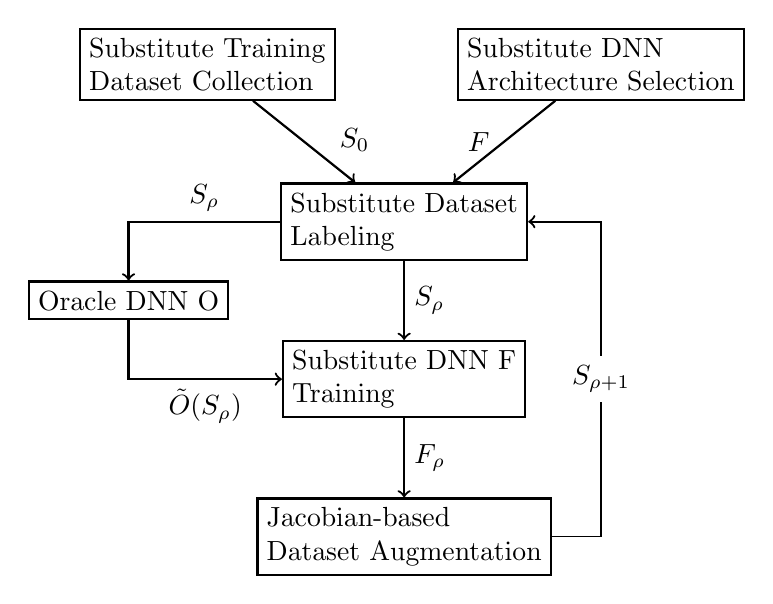
\begin{tikzpicture}[node distance = 2cm, auto]
    \node [rectangle, thick, draw, align=left] (init) at (1,10) {Substitute Training \\ Dataset Collection};
    \node [rectangle, thick, draw, align=left] (selection) at (6,10) {Substitute DNN \\ Architecture Selection};
    \node [rectangle, thick, draw, align=left] (labeling) at (3.5,8) {Substitute Dataset \\ Labeling};
    \node [rectangle, thick, draw, align=left] (training) at (3.5,6) {Substitute DNN F \\ Training};
    \node [rectangle, thick, draw, align=left] (augmentation) at (3.5,4) {Jacobian-based \\ Dataset Augmentation};
    \node [rectangle, thick, draw, align=left] (oracle) at (0,7) {Oracle DNN O};
    \node (helper) at (6,6) {$S_{\rho+1}$};

    \draw[->, thick] (init) -- (labeling) node [near end] {$S_0$};
    \draw[->, thick] (selection) -- (labeling) node [above,near end] {$F$};
    \draw[->, thick] (labeling) -- (training) node [midway] {$S_\rho$};
    \draw[->, thick] (training) -- (augmentation) node [midway] {$F_\rho$};
    \draw[->, thick] (labeling) -| (oracle) node [near start, above] {$S_\rho$};
    \draw[->, thick] (oracle) |- (training) node [near end, below] {$\tilde{O}(S_\rho)$};
    \draw (augmentation) -|  (helper);
    \draw[->, thick] (helper) |- (labeling);
\end{tikzpicture}
	\caption{\textbf{Basic flow of the Jacobian-based Dataset Augmentation.} \cite{papernot2017practical}}
	\label{fig:jbda}
\end{figure}

More precisely, the Jacobian-based dataset augmentation involves multiple training iterations, as shown in Figure~\ref{fig:jbda}.
Starting from an initial dataset $S_0$ and a selected architecture $F$, the labels of the initial iteration $\rho = 0$ are gathered.
Then, a substitute DNN $F$ is trained which is then augmented according to its Jacobian which is the gradient with respect to each input dimension.
In subsequent iterations, this dataset is further augmented until the maximum number of iterations is reached.
The substitute model which has been trained in the last iteration is the final output.

After initial experiments, we quickly noticed that the original algorithm does not produce acceptable results as-is and that it needs some refinement in our context.
Thus, we created a custom extension to this algorithm which we expect yield a better approximation of the remote decision boundary.
As previously described, the original Jacobian-based dataset augmentation takes a single image per class, fetches the remote labels, trains an intermediate model on this data and computes new synthetic data points along the gradient of the local model.
We found it problematic that firstly, this does not handle low-confidence source samples very well: The intermediate model can be hardly trained on these inputs.
Secondly, the original algorithm starts at an unknown confidence and generates new data in both the positive and negative gradient direction.
It is parameterized by a number of iterations $\rho$ and a step size $\lambda$ which are fixed for all classes.
Obviously the combination of an unknown starting point and a fixed step size in both directions is counter productive, since this can easily lead to generated images which are off the manifold and there is no way to control how many of these samples are generated.

To cope with these flaws, we modified the algorithm such that it starts with a specified number of input samples per class, which are guaranteed to be classified with a higher confidence than a certain threshold.
After that, our modified version only generates synthetic data along the negative gradient.
This reflects starting at the peak for each class and systematically exploring the path towards the minimum confidence of the model.
We also noticed that some classes never result in high confidence predictions which is why we introduced a third variable limiting the number of tries to fetch high confidence samples.
The modified algorithm always keeps track of the best samples fetched so far which are taken if the maximum number of tries has been reached.
This limit is important due to the enforced request delay of one second between each prediction.
The number of samples per class, the confidence threshold as well as the maximum number of tries per class and sample are configurable parameters in our algorithm.
Notably, by parameterizing the number of starting images per class, we improved the initial intermediate model's training results. 
Facing 43 classes (or 36 in the reduced dataset as discussed below), the training on single images per class hardly ever converged.
Moreover, we wanted to prevent overfitting on certain source images and their synthetic derivatives by this measure, since there are also different angles and lighting settings in the reference dataset.

Given the fact that the remote model has been trained on the GTSRB dataset, we had the hypothesis that it should be able to predict all occurring classes.
Since this assumption needed validation, we chose to crawl each image of the dataset once and cache the predictions in a python pickle file.
We then analyzed the results and recognized that there are seven classes of GTSRB that never occur in the classification output of the remote model:
\begin{enumerate}
	\item einseitig (rechts) verengte Fahrbahn
	\item Lichtzeichenanlage
	\item Kinder
	\item Schnee- oder Eisglätte
	\item Ausschließlich links
	\item vorgeschriebene Fahrtrichtung (geradeaus und rechts)
	\item vorgeschriebene Fahrtrichtung (geradeaus und links)
\end{enumerate}
Concluding that it would be not sensible to target these classes, we excluded them from all further considerations.
Also, the cached dataset predictions are the basis for a static map which translates the class numbers and names of the local dataset to the ones returned by the remote model.

\begin{figure}
	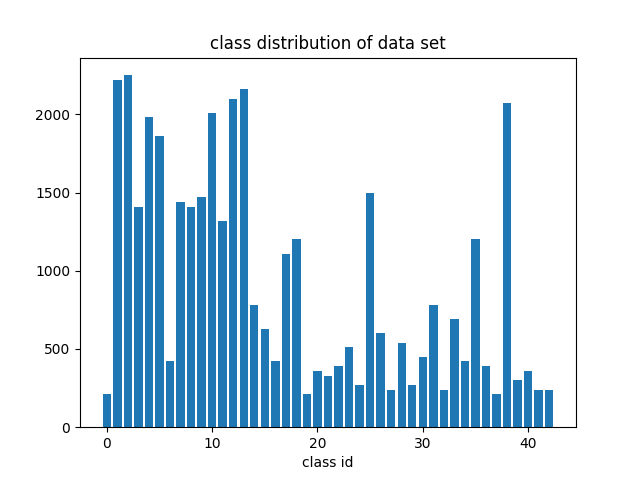
\includegraphics[width=1.1\linewidth]{figs/class_distr}
	\caption{The class ditribution of the GTSRB dataset.}
	\label{fig:class_distr}
\end{figure}

During the training set analysis, we identified an additional potential issue: the unequal number of training samples per class.
This relates to the first model stealing approach in which we rebuild a model based on the same reference dataset.
As shown in Figure~\ref{fig:class_distr}, the number of samples per class varies by order of magnitude.
We therefore also consider dataset augmentation by rotating, zooming, shearing and shifting images which are simple transformations that are guaranteed to produce valid images (if the parameters are kept in a sensible range).
As will be later discussed in subsection~\ref{subsec:backend}, we provide this optional augmentation, enhancing the reference dataset to be more balanced.

\subsection{Carlini \& Wagner}\label{subsec:cwl2}
In the following, the Carlini and Wagner $L_2$ attack is going to be recapitulated, following the ideas and notation of the original paper \cite{carlini2017towards}.
The attack has been designed with the intention of evaluating a DNN classifier's robustness by proving its upper bound.
In their paper, \citeauthor{carlini2017towards} refer to the commonly used $L_0$, $L_2$ and $L_\infty$ norms and construct an attack for each of them.
The second one of these attacks produces the least noticeable adversarial examples, which is why we chose it in this work.
As shown in Equation~\ref{eq:cwl2_min}, the attack algorithm solves an optimization problem which minimizes the distance between the original and the perturbed image while ensuring a certain target class as the output~\cite{carlini2017towards}.
Furthermore, they compute the distance in the tanh space to automatically scale the possible outputs to the range of valid pixel values as shown in Equation~\ref{eq:delta_tanh}.

\begin{equation}\label{eq:cwl2_min}
\min ||\delta||^2_2 + c \cdot f(x + \delta)
\end{equation}

\begin{equation}\label{eq:delta_tanh}
\delta = \frac{1}{2}(\tanh(w)+1) - x
\end{equation}

\begin{equation}\label{eq:cwl2_min_final}
\min ||\frac{1}{2}(\tanh(w)+1)-x||^2_2 + c \cdot f(\frac{1}{2}(\tanh(w)+1)
\end{equation}

Because the minimization is hard to compute directly for the highly non-linear functional dependency of a model, \citeauthor{carlini2017towards} substitute this by an objective function $f$ which is to be solved instead.
It ensures that the classification of the adversarial example is the target class if and only if the objective function $f$ is less than or equal to zero.
In other words, minimizing $f$ benefits the adversarial goal of a targeted misclassification.
Therefore, the optimization problem can be reformulated such that its solution is easier to compute, as depicted in the final formulation by \citeauthor{carlini2017towards} in Equation~\ref{eq:cwl2_min_final}.
They conclude that for a suitable $c > 0$, the optimal solution of the latter formulation matches the optimal solution of the former.

\subsection{Modified Carlini \& Wagner}\label{subsec:cwl2_mod}

Modification of \cite{carlini2017towards} inspired by \cite{eykholt2018robust}

\begin{equation}
\min ||\delta||^2_2 + \frac{c}{|T|} \cdot \sum_{T_i \in T} f(T_i(x + \delta))
\end{equation}

The modification of the Carlini \& Wagner attack is motivated by the context of the competition:

In a real world scenario the classification of traffic signs is done under various environmental influences.
These include but are not limited to distance and angle to the object, lighting, weather or vandalism of the sign.
Often, a small change of these factors overshadows the adversarial perturbation. % TODO citation needed
For an adversarial example to be successful, one often has to stay at the exact same position for which the sample was generated. 

\citet{eykholt2018robust} try to combat these influences with a robust physical framework for their attack.
Amongst other methods they apply multiple transformations $T_i \in T$ to their source image,
thus optimizing the perturbation to simultaneously work on multiple variations of the source image.

For our modification of the Carlini \& Wagner attack, we use four different transformations,
which mimic the classification from multiple angles: Left, slightly left, slightly right and Right.
These transformations are inspired by the InformatiCup's introductory example:
An autonomous car is driving behind a lorry, on which an adversarial sticker is placed.
This image has to fool the classifier from multiple angles to successfully yield misbehavior of the self-driving car.
While these image transformations are not sufficient enough to protect against other environmental influences, they nevertheless increase the robustness of the adversarial attacks and simulate a real-world usage.

\subsection{Robust Physical Perturbations}\label{subsec:robustphysical}

The Robust Physical Perturbation (RP$_2$) was introduced by \citet{eykholt2018robust}.
\footnote{The corresponding GitHub repository can be found in \cite{rp2repo}}

\begin{equation}
\argmin_\delta \lambda ||M_x \cdot \delta||_2 + J(F(x_i + M_x \cdot \delta), y)
\end{equation}

The original method contains a few additional operations such as a Non-Printability Score (NPS) and calculating the mean over multiple transformations -- like we adapted for our Modified Carlini \& Wagner attack.
However, we did not receive favorable results with these additional terms and subsequently removed them from the optimization.
Thus, we focused on the most important aspect of this attack, which is the ability to define a masking on the image.
This enables an attacker to define a graffiti-like perturbation.

In the original paper, this was used to reliably cause a neural network into misclassifying physical stop signs.
The InformatiCup explicitly excluded the misclassification of traffic sign images from the competition.
Yet we think this is a realistic and dangerous threat to autonomous driving as attacks can be hidden in graffiti-like perturbations as shown in Figure \ref{fig:stopsign}.

\begin{figure}[h]
\centering
\begin{subfigure}{.19\linewidth}
  \centering
  
\includegraphics[width=0.7\linewidth]{imgs/stopp_to_7}
\end{subfigure}
\begin{subfigure}{.19\linewidth}
  \centering
  
\includegraphics[width=0.7\linewidth]{imgs/7_real}
\end{subfigure}
\caption{Stop-sign (left) which is misclassified as 'Zulässige Höchstgeschwindigkeit (70)': 99.10\%; true class image (right) for comparison}
\label{fig:stopsign}
\end{figure}

\subsection{Software Development}\label{subsec:sw_development}
The development velocity, code quality and maintainability of a program are heavily dependent on applying software development techniques properly.
But also, these techniques serve the developer and not vice versa which is why we chose an appropriate degree of sticking to given techniques versus being unrestrictedly productive.
Though, given the overall situation of having too little time for too many possible features, we had to plan a suitable architecture and preselect a set of features we would like to implement on the system level.
We identified trying to implement too many features as the greatest risk for our project, which may result in a lack of focus and an overall mediocre software quality.
Since on the other hand planning everything in advance is hardly possible, we decided to employ a flexible software design and pursue a more agile approach for the integration and component level.
Employing a clear separation between the main components, we were able to focus on each system component separately and to achieve the primary goal of a successful misclassification first and to then re-evaluate which exact feature set is still realizable in the remaining time.
The final set of functional system requirements is as follows, being sorted from most to least important:
\begin{enumerate}
	\item[1.] \textbf{Misclassification}
	The software shall be able to reproducibly generate adversarial examples that are classified as traffic signs by the remote model.
	\item[2.] \textbf{CleverHans Integration}
	The software shall incorporate an interface to the CleverHans library and shall use it for attacking a model. Custom attack modifications shall be implemented using the same interface.
	\item[3.] \textbf{Website}
	The software shall provide a user-friendly front end in the form of a website.
	\item[4.] \textbf{Docker}
	The software shall be distributed using docker.
\end{enumerate}

This methodology ensured a fully functional business logic before spending time on optional tasks.
Due to the small team size of two people, we refrained from creating time-consuming documents like a formal specification and decided to meet up at least once a week to reason about the current state and which steps to take next.

When working with multiple developers on the same code base, there must be a defined flow for how to implement new features and integrate them into the code base.
We decided to use git as a source code management system and to follow the \enquote{git flow}~\footnote{This concept has been initially presented in a blog post \cite{gitflow} but has found broad application under practitioners since then.}.
A basic concept of this flow is to employ a master branch for releases, an integration branch for merging new features and short-living topic branches for the actual feature implementation.
We refined this by a custom merging strategy which is further detailed in the next subsection.

\subsection{Software Testing}\label{subsec:sw_testing}
Software testing defines a set of techniques to ensure code quality and the coherence of specification and implementation.
Applying meaningful tests reduces the technical debt in the software's life cycle and therefore decreases the time spent on fixing errors as well as the amount of unknown software bugs.
Which exact techniques to apply must be decided for each project individually and depends on multiple factors like whether there are stakeholders interested in the outcome of a test and the benefit cost ratio.
For example, setting up an extensive framework for regression testing is not sensible in our context because there is only a single release version, after which the won't be any further releases requiring a regression.
Even unit tests do not fit our project very well because of the constantly changing code base which would incur the cost of permanently adjusting the test cases and re-evaluating if they are still meaningful.
Also, having no clearly defined requirements, it is not possible to derive a test plan and specification, rendering most testing approaches ineffective.
We therefore restricted ourselves to the following three testing techniques which we found appropriate in our context:
\begin{description}
	\item[Informal Code Review] This is a form of static testing which we applied before merging new features. To maintain a high development velocity, we chose the following flow: For a finished feature, the code author notifies the reviewer who then checks out the feature branch, reviews the changes and executes the code. The reviewer accepts or rejects the changes depending on potential open issues. On acceptance, the branch is merged and sent back for re-iteration on rejection. The reviewer also has the opportunity to ask for a peer review if there are many open questions or if the amount of changes is too large.
	\item[Peer Review] For bigger sets of changes, we held dedicated sessions in which the reviewer examined each change, pointing out discrepancies and asking questions. The code author then provided an explanation or noted this aspect as an open issue. After solving all issues and implementing the fixes, the reviewer checked it again before merging in an informal review.
	\item[Scenario-based Testing] This testing technique applies to the system level and defines scenarios to be tested. We identified this as vital to ensure that all components are well-integrated and that there are no unforeseen errors at the end. Testing scenarios helps ensuring a good user experience which is our main non-functional requirement in the context of this competition. 
\end{description}
Enforcing this testing strategy, we were able to develop with a high developing velocity\footnote{We performed a total of ca. 170 commits and an average of $1.1$ commits per day and team member (metrics taken from our git repository over the whole span of the project).} while maintaining a reasonable code quality.

%!TEX root = paper.tex

% Software architecture, not CNN-architecture
\section{Architecture}\label{sec:arch}

This section describes the general architecture of our software solution and reasoning for choosing specific tools.
We begin by describing the website front end which is visible to the user.
From there on we move to the server's back end and finally into our business logic consisting mainly of independent python programs.

We chose python as our main programming language, because of its extensive usage and support in machine learning -- especially the TensorFlow framework.
We decided to build a website as our main user interface and subsequently chose the Django Framework to easily integrate our python programs into the server back end.
Considering the attack algorithms, we selected the CleverHans library because it provides a unified interface to a variety of attacks.
By using a website as the front end, our user interface is largely platform independent and nicely separated from our back end, which we provide via a REST API.
Also, the web context allows us to use existing techniques to provide a visually appealing and responsive design.

Currently, our website is a local single user system, which we distribute as a docker container.	
We leave the thorough security evaluation and multi-user management to future extensions and focus more on generating strong adversarial examples.
Though, using docker containers and a clear separation of the front end, the HTTP request management as well as our business logic, our architecture makes these extensions feasible.
This separation has been strictly implemented which furthermore allows experienced users to connect to the docker container's TTY and use the python script back end directly without starting the web server.

% TODO: Jonas, was meinst du? Ich würde das einfach weglassen. Das klingt nach einer Rechtfertigung.
%This decision was mainly influenced by the competition's setup and further drawbacks of %hosting a public server.
%If we had hosted our server publicly, we had to place additional emphasis on security %evaluation, multi-user accessibility and server configuration.
%We therefore decided on a local container deployment.
%
\subsection{Front End}\label{subsec:frontend}

The front end is divided into two categories: \enquote{Models} (model creation) and \enquote{Attack}.
In the former category, the user is able train, steal, upload and generally manage models. The latter is then used to configure and start attacks on a model.
All information in this subsection relates to the client-side part of our application: HTML documents, CSS stylesheets, JavaScript files and other static content.

\subsubsection{Design Principles}
The main goal for the front end is a visually appealing and responsive design.
This includes the scalability of the website across different screen sizes and even device types.
Therefore, all DOM object properties are defined using relative sizes, i.e. \enquote{em} for the size relative to the parent element or \enquote{vh} for the size relative to the view port size.
We also leverage the twitter bootstrap framework for a scalable base design\footnote{\url{https://getbootstrap.com/}} as well as a bootstrap wrapper theme\footnote{\url{https://bootswatch.com/darkly/}} which we found suitable for a hacking-related competition.

A second requirement is a user-friendly flow.
This includes a unified layout across multiple subdomains and expressive icons for which we used the free icons from fontawesome\footnote{\url{https://fontawesome.com/}}.
Moreover, this design goal implies low latencies after clicking a button and an immediate visual feedback, which is solved by our REST API and asynchronous requesting(see~\ref{subsec:webserver}).
The user's orientation on the page is further supported by hovering effects in potentially large tables.
Finally, a user-friendly design also means preventing the user from taking possibly inadvertent actions like deleting a trained model which took multiple hours to train.
We thoroughly implemented these design goals in all the below described parts of the website.

The HTML documents are dynamically generated using the Django template system.
This allows for having a static templates which are filled according to a given context: For example, the table of available models is dynamically created with respect to the prevalent models in the docker container.
Also, this drastically decreases code duplications: The templates support inheritance which allowed us to define a base layout in a root template which is inherited from by each other template.
As a consequence, a change in e.g. the navigation bar would only affect a single file, which reduces the risk of code inconsistencies.

\subsubsection{Welcome Page}
The welcome page is intended to show an inviting and motivating starting page with a quick navigation to the two main parts of the front end.
It explains in simple words what to expect there and employs a minimal design.

\subsubsection{Models -- Overview}
As discussed in Section \ref{sec:methodology}, for an attack to be possible, we need to train a local substitute model.
The model overview tab contains all available models as well as their meta-data (name, size, date of last modification, architecture).
Clicking on the info icon shows a modal containing a detailed overview about the model's layers.
The user can choose to attack one of the trained models and is redirected to the attacking section accordingly. 
Furthermore, the user is able to upload own models on this page.
The trash icon triggers deleting a model.
Referring to the above described design principles, the website prompts for a second approval before actually performing the request to prevent deleting a model by accident.

\subsubsection{Models -- Training}
This page enables the user to configure and start a new training phase of a substitute model. 
Since training a model is very resource intensive, we prevent multiple simultaneous training processes.
The page itself consists of a form which collects all training parameters.
We chose to provide default values which yielded the best results in our experiments, effectively supporting a potentially less-experienced user.

\subsubsection{Models -- Details}
This page displays the details of the current training process and enables a user to abort the running training phase.
To show the live console output, a script is polling the internal state of the respective standard output (stdout) file descriptor via our REST API. 
If there is no process in progress, an appropriate message is shown.


\subsubsection{Attack -- Overview}
Similar to the model overview, this page contains a table to manage the different attacks.
The shown entities in this context are the performed runs: Each started attack is identifiable by its process ID (PID) and the console output can be reviewed live or in retrospective.
If an attack run is not needed anymore, it can be removed from the table using the trash icon.

\subsubsection{Attack -- Attack}
This tab offers starting a new attack on a source image.
The form fields update according to the selected attack algorithm because not all approaches use the same set of parameters.
Also, the user is prompted to upload an image which is then taken to attack the selected model.
Starting multiple attacks simultaneously is supported here since these are less resource intensive.
An error alert may show up if any invalid form data had been passed.
For example, loading a source image which is not 64 by 64 pixels in size results in such an error.

\subsubsection{Attack -- Details}
This tab works almost exactly like the model details except for that it additionally shows the classification result of the source and generated images.
Thus, it enables the user to evaluate her attack after it has finished.
Also, the generated images are shown on this page which enables the user to download them by right-clicking and saving them.

Attack:
\begin{enumerate}
\item path('', views.overview, name='index'),
\item path('index.html', views.overview),
\item path('overview.html', views.overview),
\item path('details.html', views.details),
\item url('attack.html', views.attack),

	%# GET
	%url('proc_info', rest.handle_proc_info),
	%url('list_images', rest.handle_list_images),
	%url('classify', rest.handle_classify),

	%# POST
	%url('start_attack', rest.handle_start_attack),
	%url('delete_proc', rest.handle_delete_proc)
\end{enumerate}

Model:
\begin{enumerate}
\item path('', views.overview, name='index'),
\item path('index.html', views.overview),
\item path('overview.html', views.overview),
\item path('training.html', views.training),
\item path('details.html', views.details),

	%# GET
	%url('model_info', rest.handle_model_info),

	%# POST
	%url('deletemodel', rest.handle_delete_model),
	%url('uploadmodel', rest.handle_upload_model),

	%url('start_training', rest.handle_start_training),
	%url('abort_training', rest.handle_abort_training),
\end{enumerate}

\begin{enumerate}
\item Pipeline-artig
\item Durch Weboberfläche konfigurierbar
\end{enumerate}

\subsection{Django Server}\label{subsec:webserver}
The Django server acts as a blend of web and application server.
It serves static content like style sheets and HTML documents and responds to HTTP requests.
We leveraged Django's middleware capabilities to automatically serve the static content and dispatch HTTP requests.
As a result, we only had to implement the responses to the HTTP GET and POST requests.
In general, we decided to implement a REST API in which GET requests are used to ask for the state of certain resources which are identified by an URI.
These requests are idempotent, meaning that successive identical GET requests yield the same server responses (as demanded by RFC 7231\cite{rfc7231}).
All state-changing actions are implemented as POST requests, for which an CSRF protection token is sent along with the generated HTML page.

The request handling code does not contain any further logic except for parsing the requests and some basic input validation which is used to display the respective error message in case of invalid request data.
We decided for a design with server-side input validation which would be a critical security requirement in future extensions supporting hosting the website over a network.
These handlers issue other python scripts, which also work in a standalone mode.
This is the manifestation of the previously described strict separation of duties.

Regarding the code separation, each main component is realized as a separate \enquote{Django App}: This is Django's mechanism for grouping sub-components.
We identified three main components in our software which are implemented as separate Django Apps: welcome, models and attack.
This grouping is reflected in the HTML templates, JS scripts and CSS files, which increases the interchangeability of components and the enforcement to use clear interfaces.

For actions that require a lot of processing like training or attacking a model, we employed a special mechanism for handling asynchronous sub-processes.
In order to organize these, we leverage the existing operating system process management.
An overview about the information flow is presented in Appendix~\ref{app:doublefork}.
When the user issues a start command (either training or attack), a new process is spawned and the website receives an immediate response whether starting the process has been successful.
Then, a JavaScript \enquote{setInterval} function periodically polls the state of the process.
To test whether a process is still running, the Django middleware emits a KILL(0) system call which is successful if there exists a running process with the specified PID and errors otherwise.
However, we need to apply a small trick to be able to use this mechanism which is known as \enquote{double fork}: To spawn an asynchronous worker process, we first fork an intermediate process that again forks the target process, returns its PID to the parent (Django handler) and then exits.
Due to the behavior of the operating system, the worker process is now a child of the init process (PID 0), which takes care of terminating the process after completion automatically.
This is important to prevent zombie processes because these would remain as \enquote{defunct} processes in the process table of the operating system, until the parent process (Django) exits.
Since we don't want to restart the web server because a sub-process has finished, we applied this double fork technique.
The advantage of this setup is that we leverage existing operating system mechanisms and don't have to re-implement this ourselves which might not cover all edge cases.

\subsection{Python Back-End}\label{subsec:backend}
The python back end represents our business logic and is realized as a set of standalone scripts for the main tasks, some auxiliary scripts and a small configuration file which defines common variables like the path to the cache directory.
Considering the standalone scripts, each of them realizes a high level function like starting a training, an attack or crawling the remote predictions for a dataset.
They expose all internal parameters as command line arguments such that they can be either called by hand or by the above described sub-processing mechanism.
Whenever there are commonly used functions between these scripts, an auxiliary script has been created to avoid code duplication which implements the DRY\footnote{DRY = \enquote{don't repeat yourself}} software developing principle.

An example for an auxiliary script is \enquote{gtsrb.py}, which collects all properties of the reference dataset and provides functions to retrieve the data as well as plotting distributions over the different classes.
This encapsulates all information and functions belonging together into a single script and provides them over an interface.
If we were to manipulate data on a different reference dataset in the future, we would only have substitute this file with a similar one containing the information for the new dataset.
As a consequence, many of the internal scripts are interchangeable which greatly improves the maintainability and extensibility of our program.

Regarding the choice of programming language, there have been three main factors which emphasized why python would be the best choice in our case:
\begin{description}
	\item[Scripting Language] This type of language allows for writing very expressive and succinct code, which helps at implementing features fast while avoiding boiler plate code. 
	A shorter source code is easier to maintain and fewer lines of code are also likely to contain fewer bugs~\cite{jain2017clairvoyant}. 
	Considering the small time frame of the competition, this outweighs possible drawbacks like the missing error checking at compile time.
	\item[Packet Management System] The python package management system \enquote{pip} incorporates all required dependencies in the default sources and allows for easily maintaining them on a project level using virtual environments. 
	Utilizing widely used  and mature packets like Django or CleverHans, we are confident that these dependencies impose only a small risk of introducing bugs.
	\item[Developer Experience] Developers write better code in languages they are highly familiar with.
	Since this is the case for both team members, we preferred this choice over other equally good solutions.
\end{description}

\subsection{Docker Setup}
Docker is a commonly used containerization and virtualization engine.
It provides the opportunity to bundle a program and all its dependencies into a single container which then may be run on different operating systems.
The result is an easy to install software with the only requirement using the same kernel.
Also, completely uninstalling a program with all its dependencies becomes an easy task with docker containers.
This technology therefore greatly simplifies distributing software and avoiding situations in which it works on a developer's machine but not on the user's.
For the final submission, we choose to offer two options.
First, we provide a \enquote{Dockerfile} and the git repository, which the user may use to create a docker image herself and instantiate a container.
Second, we also distribute a ready-to-run docker container incorporating a copy of the repository.

Having a closer look on the container, one might recognize that it is distributed without the reference dataset (GTSRB) and external dependencies (pip packages, twitter bootstrap etc.).
We decided to reduce the size of the container and separate the code from the data as much as possible.
Subsequently, there exists a setup shell script which will download all required data and put it in a so called \enquote{DATA\_ROOT} on startup of the container.
This data root is a directory that can be mounted into the docker container such that, on a potential software update, the user would only need to replace the docker container and can then immediately continue working as before.
A further benefit of this is that all relevant information concerning the program's state is also saved there which implies that the user could update the software without data loss.
Considering that training models and fetching predictions is a very time-consuming task, we wanted to ensure that the user has to perform these tasks not more than once.

Finally, the virtualization aspect of docker enables us to leverage operating system features like system calls and allowing a web application to write files without the risk of harming the host environment.
For example, docker employs strict policies preventing containers from accidentally (or intentionally) modifying host files with the exception of mounted directories (like the data root).
From a security perspective, it is also valuable to only expose a single port to the host network which is the one used to serve the website.


%!TEX root = paper.tex

\section{Results}

In this section we present and discuss our five submitted images. The images have been generated from the source images which are shown in Figure \ref{fig:source_images}.

Alongside each submitted image we appended a .conf file which contains the exact command line call which was used to generate the respective image. The submitted images are shown in Figure \ref{fig:submitted}. For comparison an image of the target classes is displayed beneath each of them.

\begin{figure}
\centering
\begin{subfigure}{.19\linewidth}
  \centering
  
\includegraphics[width=0.7\linewidth]{imgs/octocat}
\end{subfigure}
\begin{subfigure}{.19\linewidth}
  \centering
  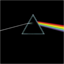
\includegraphics[width=0.7\linewidth]{imgs/darkside}
\end{subfigure}
\begin{subfigure}{.19\linewidth}
  \centering
  
\includegraphics[width=0.7\linewidth]{imgs/gi}
\end{subfigure}
\begin{subfigure}{.19\linewidth}
  \centering
  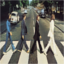
\includegraphics[width=0.7\linewidth]{imgs/abbey}
\end{subfigure}
\begin{subfigure}{.19\linewidth}
  \centering
  
\includegraphics[width=0.7\linewidth]{imgs/die_???}
\end{subfigure}
\caption{Source images}
\label{fig:source_images}
\end{figure}

\begin{figure}[!h]
\centering
\begin{subfigure}{.19\linewidth}
  \centering
  
\includegraphics[width=0.7\linewidth]{imgs/4}
\end{subfigure}%
\begin{subfigure}{.19\linewidth}
  \centering
  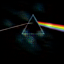
\includegraphics[width=0.7\linewidth]{imgs/7}
\end{subfigure}
\begin{subfigure}{.19\linewidth}
  \centering
  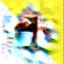
\includegraphics[width=0.7\linewidth]{imgs/10}
\end{subfigure}
\begin{subfigure}{.19\linewidth}
  \centering
  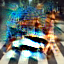
\includegraphics[width=0.7\linewidth]{imgs/16}
\end{subfigure}
\begin{subfigure}{.19\linewidth}
  \centering
  
\includegraphics[width=0.7\linewidth]{imgs/20}
\end{subfigure}

\begin{subfigure}{.19\linewidth}
  \centering
  
\includegraphics[width=0.7\linewidth]{imgs/4_real}
\end{subfigure}%
\begin{subfigure}{.19\linewidth}
  \centering
  
\includegraphics[width=0.7\linewidth]{imgs/7_real}
\end{subfigure}
\begin{subfigure}{.19\linewidth}
  \centering
  
\includegraphics[width=0.7\linewidth]{imgs/10_real}
\end{subfigure}
\begin{subfigure}{.19\linewidth}
  \centering
  
\includegraphics[width=0.7\linewidth]{imgs/16_real}
\end{subfigure}
\begin{subfigure}{.19\linewidth}
  \centering
  
\includegraphics[width=0.7\linewidth]{imgs/20_real}
\end{subfigure}
\caption{Submitted images}
\label{fig:submitted}
\end{figure}

\begin{enumerate}
\item
\textbf{Überholverbot für Kraftfahrzeuge aller Art: 99.99 \%}

The first adversarial example was generated from Git\-Hub's octocat using the Carlini \& Wagner L2 algorithm on a substitute model,
which was trained on the GTSRB training data.
It does not resemble the target sign at all and the source image is clearly recognizable.

\item
\textbf{Zulässige Höchstgeschwindigkeit (70): 99.41\%}

The second example was generated from the album cover of Pink Floyd's "The Dark Side of the Moon".
It uses the same setup as the first image.
Although there exists some noise on the black background, the target image is not recognizable and the album cover is still clearly visible.

\item
\textbf{Gefahrenstelle: $\approx$100\%}

\begin{figure}[!h]
\centering
\begin{subfigure}{.19\linewidth}
  \centering
  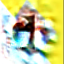
\includegraphics[width=0.7\linewidth]{imgs/robust_10/0_ll}
  \caption{99.97\%}
\end{subfigure}
\begin{subfigure}{.19\linewidth}
  \centering
  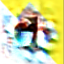
\includegraphics[width=0.7\linewidth]{imgs/robust_10/1_l}
  \caption{$\approx$100\%}
\end{subfigure}
\begin{subfigure}{.19\linewidth}
  \centering
  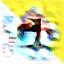
\includegraphics[width=0.7\linewidth]{imgs/robust_10/2_c}
  \caption{95.03\%}
\end{subfigure}
\begin{subfigure}{.19\linewidth}
  \centering
  
\includegraphics[width=0.7\linewidth]{imgs/robust_10/3_r}
  \caption{99.85\%}
\end{subfigure}
\begin{subfigure}{.19\linewidth}
  \centering
  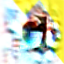
\includegraphics[width=0.7\linewidth]{imgs/robust_10/4_rr}
  \caption{99.98\%}
\end{subfigure}
\end{figure}

The third adversarial example is based on the GI logo.
It was constructed using the modified Carlini \& Wagner attack,
which modifies an image from multiple perspectives simultaneously.
The attack was performed on the model, which was trained using Jacobian based dataset augmentation.

The generated images are heavily perturbed;
yet, the GI logo is still noticeable while the target class is not recognizable.

\item
\textbf{Wildwechsel: 100\%}

\begin{figure}[!h]
\centering
\begin{subfigure}{.19\linewidth}
  \centering
  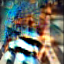
\includegraphics[width=0.7\linewidth]{imgs/robust_16/0_ll}
  \caption{97.62\%}
\end{subfigure}
\begin{subfigure}{.19\linewidth}
  \centering
  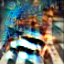
\includegraphics[width=0.7\linewidth]{imgs/robust_16/1_l}
  \caption{100\%}
\end{subfigure}
\begin{subfigure}{.19\linewidth}
  \centering
  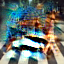
\includegraphics[width=0.7\linewidth]{imgs/robust_16/2_c}
  \caption{100\%}
\end{subfigure}
\begin{subfigure}{.19\linewidth}
  \centering
  
\includegraphics[width=0.7\linewidth]{imgs/robust_16/3_r}
  \caption{100\%}
\end{subfigure}
\begin{subfigure}{.19\linewidth}
  \centering
  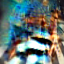
\includegraphics[width=0.7\linewidth]{imgs/robust_16/4_rr}
  \caption{99.99\%}
\end{subfigure}
\end{figure}

The fourth adversarial example uses the same attack as the third, but is performed on the GTSRB-model.
It was generated from the Beatle's "Abbey Road" album cover.

Though the zebra crossing is still visible on closer inspection, the original image is too heavily perturbed to be identifiable. 
Nevertheless, the adversarial example does not resemble the target class (nor any other traffic sign) and is therefore valid.

\item
\textbf{Vorfahrt: 99.99\%}

\begin{figure}[!h]
\begin{subfigure}{.19\linewidth}
  \centering
  
\includegraphics[width=0.7\linewidth]{imgs/die_???}
  \caption{Source}
\end{subfigure}
\hspace{0.05\linewidth}
\begin{subfigure}{.19\linewidth}
  \centering
  
\includegraphics[width=0.7\linewidth]{imgs/inv_???mask}
  \caption{Mask}
\end{subfigure}
\hspace{0.05\linewidth}
\begin{subfigure}{.19\linewidth}
  \centering
  
\includegraphics[width=0.7\linewidth]{imgs/20}
  \caption{Result}
\end{subfigure}
\end{figure}

The last image was created by the robust physical attack (RP$_2$) applied to the GTSRB-model.
It was generated from the logo of the three investigators (Die Drei Fragezeichen) where the question marks have been masked (i.e. they remain unperturbed).
The final image is not recognizable as a traffic sign.

\end{enumerate}

%!TEX root = paper.tex"`

\section{Model architecture}

\begin{enumerate}
\item Aufbau CNN\footnote{\url{https://chsasank.github.io/keras-tutorial.html}}

\begin{table}[!h]
\centering
\begin{tabular}{ l r }
\hline

Layer Type & GTSRB Model \\
\hline

  Convolution + ReLU & $3 \times 3 \times 32$ \\
  Convolution + ReLU & $3 \times 3 \times 32$  \\
  Max Pooling & $2 \times 2$ \\
  Dropout & $0.2$ \\

  Convolution + ReLU & $3 \times 3 \times 64$ \\
  Convolution + ReLU & $3 \times 3 \times 64$ \\
  Max Pooling & $2 \times 2$ \\
  Dropout & $0.2$ \\
  
  Convolution + ReLU & $3 \times 3 \times 128$ \\
  Convolution + ReLU & $3 \times 3 \times 128$ \\
  Max Pooling & $2 \times 2$ \\
  Dropout & $0.2$ \\
    
  Fully Connected + ReLU & $512$\\
  Dropout & $0.5$ \\

  Fully Connected + ReLU & $43$\\
  
  Softmax & $43$ \\ \hline 
  \vspace{1.5pt}
\end{tabular}
\caption{Architecture of our neural networks}
\label{table:model}
\end{table}
\item Geschichte Adversarial Samples
\item Carlini \& Wagner Angriff \cite{carlini2017towards}
\item Limitation of 64x64 -> no real world attack but constructed
\end{enumerate}

%!TEX root = paper.tex"`

\section{Evaluation}

To further evaluate the quality of the attacks, we generated multiple adversarial examples with different configurations and classified them using the \textbf{remote} model. In the following we briefly discuss our setup and the selection of the attack parameters. Afterwards, we present and discuss the attack results.

\subsection{Setup}

\begin{table}
\begin{tabular}{l | l}
\textbf{Parameter} & \textbf{Values} \\\hline

target & 0,2,3,5,11,12,16,27,31,33 \\\hline

model & gtsrb\_model, jbda3\\\hline

attack & cwl2, robust\_cwl2\\\hline

image & abbey, gi, octocat\\\hline

conf & 15, 20
\end{tabular}
\caption{Attack Configuration}
\label{tab:cli_params}
\end{table}

\begin{minipage}{\linewidth}
An adversarial example is generated using the command line call:

\vspace{2ex}
\texttt{python3 attack\_model.py ----target [target]}

\hspace{4cm}\texttt{----model [model]}

\hspace{4cm}\texttt{----attack [attack]}

\hspace{4cm}\texttt{----image [image].png}

\hspace{4cm}\texttt{----confidence [conf]}

\hspace{4cm}\texttt{----max\_iterations 7500}

\hspace{4cm}\texttt{----binary\_search\_steps 12}
\vspace{2ex}
\end{minipage}

Arguments which are embraced by parentheses are taken from Table \ref{tab:cli_params}. If the Carlini \& Wagner attack (cwl2) is chosen as the attack technique, this attempts to create one adversarial example. Otherwise, if our modified Carlini \& Wagner attack (robust\_cwl2) is used, five adversarial examples are generated.\footnote{Please note, that the 'modified Carlini \& Wagner' attack from Section \ref{subsec:cwl2_mod} is internally referred to as robust\_cwl2} We omitted the Robust Physical Perturbation attack (RP$_2$) from our evaluation, because the success of the attack heavily depends on the masking image which might skew the results.

The attack\_model script only returns \emph{successful} adversarial examples, otherwise no image is generated. For the Carlini \& Wagner attack an adversarial example is successful, if the local model classifies it as the target class. The modified Carlini \& Wagner attack only returns a adversarial examples if the center image (where no perspective transformation is applied) is classified as the target class.

For our evaluation we chose ten random labels as our target class to keep the computation at a moderate level while still receiving meaningful results. The models under attack were created using the techniques from Section \ref{subsec:modelstealing}: \emph{Rebuilding} was used for the gtsrb model and \emph{Stealing} with Jacobian based dataset augmentation was used for the jbda model. 

The results of the attacks are displayed in Table \ref{tab:cwl2_result} and Table \ref{tab:robust_result}. Each cell shows the number of adversarial examples in the respective category. To illustrate this for the modified Carlini \& Wagner attack results (Table \ref{tab:robust_result}): 37 adversarial examples of the 'abbey' image (which were generated with a confidence parameter of 20 against the gtsrb model) were classified with a confidence higher than 90\% by the remote model for the target class. On the other hand, four adversarial examples did not transfer and received a target-score lower than 90\%. Recall, that the modified C\&W attack is able to produce five adversarial example in one run. Therefore, the attack is potentially able to create 50 adversarial examples for the ten given targets. Thus, 43 of the potential 50 adversarial examples were successfully created on the local model.

In the following we use the notation:

\begin{itemize}
\item[-] $P(C)$ = Probability of an adversarial example being successfully \textbf{created} on a local model
\item[-] $P(T)$ = Probability of an adversarial example \textbf{transferring} to the remote model (i.e. classification $\geq90\%$)
\item[-] $P(G)$ = Probability that the adversarial example was generated on the local \textbf{gtsrb model}
\item[-] $P(J)$ = Probability that the adversarial example was generated on the local \textbf{jbda model}
\end{itemize}

\subsection{Carlini \& Wagner}



\begin{align}
P(C) = \frac{93}{120} &= 0.775\\[1ex]
P(C \mid G) = \frac{54}{60} &= 0.9\\[1ex]
P(C \mid J) = \frac{39}{60} &= 0.65\\[1ex]
P(T \mid G \wedge C) = \frac{47}{54} &\approx 0.87\\[1ex]
P(T \mid J \wedge C) = \frac{28}{39} &\approx 0.72\\[1ex]
\end{align}

\begin{table}
\begin{tabular}{l l | r r | r r | r r}
& & abbey & & gi & & octo & \\[1ex]
& & \footnotesize$\geq90\%$ & \footnotesize$<90\%$ & \footnotesize$\geq90\%$ & \footnotesize$<90\%$ & \footnotesize$\geq90\%$ & \footnotesize$<90\%$ \\[1ex]
\hline
gtsrb & 15 & 8 & 2 & 7 & 2 & 7 & 0 \\[1ex]
& 20 & 10 & 0 & 8 & 1 & 7 & 2 \\[1ex]
\hline
jbda & 15 & 6 & 3 & 1 & 3 & 6 & 1 \\[1ex]
& 20 & 7 & 0 & 2 & 3 & 6 & 1
\end{tabular}
\caption{Results for the Carlini \& Wagner attack}
\label{tab:cwl2_result}
\end{table}

\subsection{Modified Carlini \& Wagner}

\begin{align}
P(C) = \frac{381}{600} = 0.635\\[1ex]
P(C \mid G) = \frac{232}{300} \approx 0.77\\[1ex]
P(C \mid J) = \frac{149}{300} \approx 0.50\\[1ex]
P(T \mid G \wedge C) = \frac{205}{232} \approx 0.88\\[1ex]
P(T \mid J \wedge C) = \frac{128}{149} \approx 0.86\\[1ex]
\end{align}

\begin{table}
\begin{tabular}{l l | r r | r r | r r}
& & abbey & & gi & & octo & \\[1ex]
& & \footnotesize$\geq90\%$ & \footnotesize$<90\%$ & \footnotesize$\geq90\%$ & \footnotesize$<90\%$ & \footnotesize$\geq90\%$ & \footnotesize$<90\%$ \\[1ex]
\hline
gtsrb & 15 & 36 & 7 & 30 & 2 & 34 & 5
\\[1ex]
 & 20 & 37 & 4 & 30 & 4 & 38 & 5\\[1ex]
\hline
jbda & 15 & 30 & 7 & 12 & 3 & 26 & 8
\\[1ex]
  & 20 & 23 & 1 & 14 & 1 & 23 & 1
\end{tabular}
\caption{Results for the \textit{modified} Carlini \& Wagner attack}
\label{tab:robust_result}
\end{table}

%!TEX root = paper.tex"`

\section{Extensibility}

\begin{enumerate}
\item Weitere Angriffe einbauen
\item Eigene Maske bei Physical-Attack durch Benutzer definieren
\item Mehrbenutzersystem
\item ...
\end{enumerate}

%\bibliographystyle{IEEEtran}
\bibliographystyle{plainnat}
\bibliography{bib} %name of bib file

\end{document}
